\chapter{Experiments} \label{chapter:experiments}

In this chapter, we evaluate how effective our learned cost function is, which is described below, where $D$ is the number of features, $A$ is the set of actions and the resulting value of $\mathbf{x}$ after the interventions is $\mathbf{x}^{\text{PCF}}$.

\begin{align} \label{eq:cost_function_experiments}
	\cost(A, \beta_k, \mathcal{F}) & = \sum_{i=1}^D \delta_i \beta_{ki}^2 \\ \nonumber
	A & = \big\{(\mathbf{S}, \text{do} \{\mathbf{x}_i:=\mathbf{x}_i + \boldsymbol{\delta}_i\}_{i=1, \ldots, D})\big\} \\ \nonumber
	\mathbf{x}^{\text{PCF}} & = \mathbb{I}_{i \in I} \boldsymbol{\delta}_i + \bigg( \mathbf{x}_i + f_i(\textbf{pa}^{\text{PCF}}_i) - f_i(\textbf{pa}_i) \bigg)
\end{align}

\section{End-to-End Methodology}

The end to end methodology for generating recourse with a learned cost is shown in Figure \ref{fig:workflow}, and more details on each of the steps in the methodology are described below.

\begin{figure}[!htb]
	\centering
	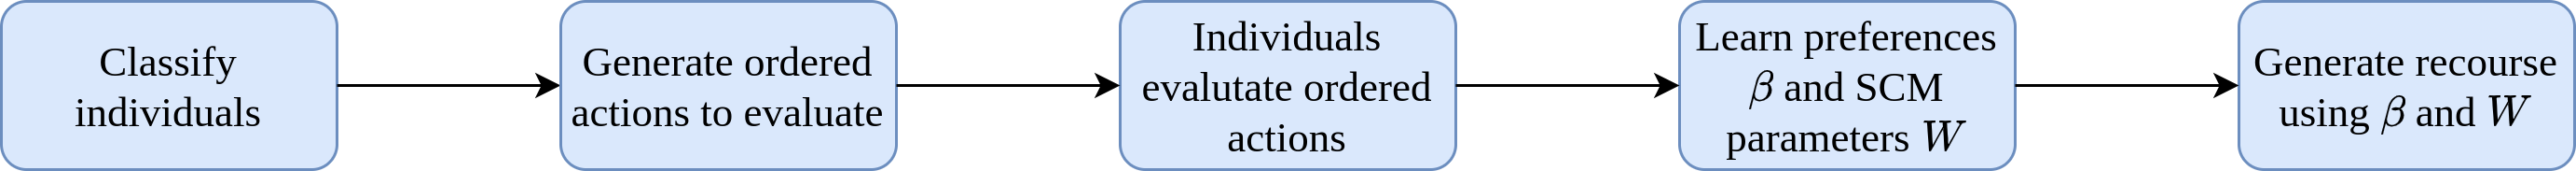
\includegraphics[width=\linewidth]{images/draw.io/workflow.png}
	\caption{End-to-End Methodology}
	\label{fig:workflow}
\end{figure}

\begin{enumerate}
	\item \textbf{Classify individuals}. Individuals with features $\mathbf{X}$ are assessed by a classifier and are classified either positively (e.g., loan approved, admission acceptance) or negatively (e.g., loan rejected, admission rejected). In this thesis, logistic regression has been used, largely for simplicity. However, as an augmented Lagrangian gradient descent optimisation is used to generate recourse (see section \ref{section:generating_recourse}), any differentiable classifier could be used instead of logistic regression.
	
	\item \textbf{Generate ordered actions to evaluate}. We randomly generate actions for each negatively classified individual and associated randomly generated orderings. This is another area for future work, where an online or Bayesian approach could be used to generate recourse actions in order to maximise information gain, such as the approach used in \textcite{detoniPersonalizedAlgorithmicRecourse2023}.
	
	\item \textbf{Users evaluate ordered actions}. Using the cost function described in equation \ref{eq:cost_function_experiments} with noisy user preferences $\tilde{\beta_k}$ and noisy SCM $\tilde{\mathcal{F}}$, users evaluate which of the ordered actions they are presented with they prefer. 
	
	\item \textbf{Learn preferences $\hat{\beta_k}$ and SCM approximation parameters $\hat{W}$}. The model deployer then learns user preferences $\hat{\beta_k}$ and a linear approximation of the true SCM $\hat{W}$ using the optimisation presented in section \ref{section:cost_learning_formulation}.
	
	\item \textbf{Generate recourse using $\hat{\beta_k}$ and $\hat{W}$}. The model deployer then generates recourse $\mathbf{X}^*$ for the negatively classified users.
	
\end{enumerate}



\section{Synthetic Data}

We create synthetic SCMs, from which we sample our data $\mathbf{X}$. We simulate two different SCMs, the first being a linear SCM and the second a non-linear SCM. In both cases, we assign individuals to have the same randomly generated feature mutability $\beta$ plus some noise. This means that individuals tend to have similar preferences, but do not have the same preferences.

\subsection{Linear SCM} \label{section:linear_scm}

Shown below are the structural equations of the linear SCM $\mathcal{M}_{\text{LIN}}$ as well as the associated causal graph.

\begin{align}
	x_1 & = u_1 & u_1 \sim N(0,1) \\ \nonumber
	x_2 & = u_2 + 0.5x_1 & u_2 \sim N(0,1) \\ \nonumber
	x_3 & = u_3 + 0.2x_1 + 0.3x_2 & u_3 \sim N(0,0.5) \\ \nonumber
	y   & \sim \text{Bernoulli}(\sigma(0.1x_1 + 0.2x_2 + 0.3x_3))
\end{align}

\begin{figure}[!htb]
	\centering
	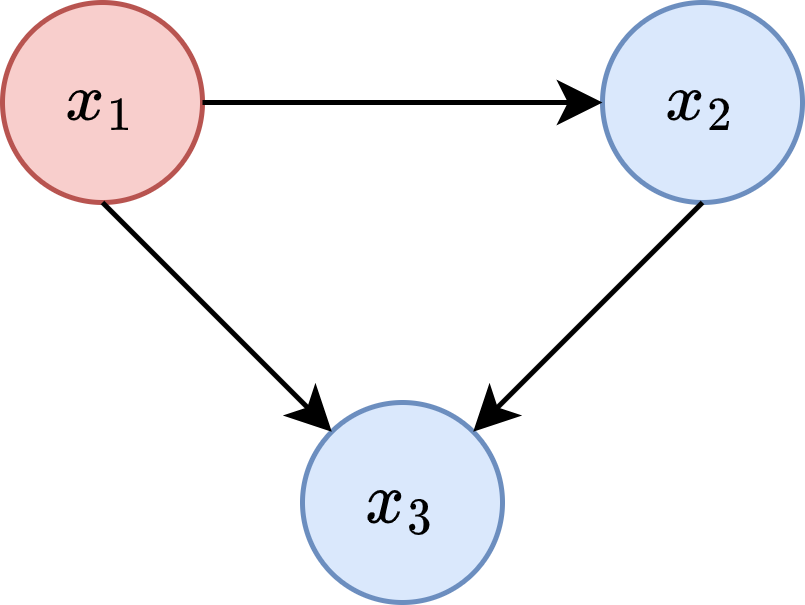
\includegraphics[width=0.4\linewidth]{images/draw.io/toy_scm.png}
	\caption{Linear SCM $\mathcal{M}_{\text{LIN}}$}
	\label{fig:simple_scm}
\end{figure}

\subsection{Non-Linear SCM}

Shown below are the structural equations of the non-linear SCM $\mathcal{M}_{\text{NL}}$ as well as the associated causal graph.

\begin{align}
	x_1 & = u_1 & u_1 \sim N(0,1) \\ \nonumber
	x_2 & = u_2 - \frac{2}{1 + x_1^2} & u_2 \sim N(0,1) \\ \nonumber
	x_3 & = u_3 + 0.2x_1 + 0.1x_1x_2 & u_3 \sim N(0,0.5) \\ \nonumber
	x_4 & = u_4 + 0.4x_1 + 0.7x_2x_3 & u_4 \sim N(0,0,5) \\ \nonumber
	x_5 & = u_5 + 0.8x_1 & u_5 \sim N(0,0.5) \\ \nonumber
	y   & \sim \text{Bernoulli}(\sigma(0.1x_1 + 0.2x_2 + 0.3x_3 + 0.4x_4 + 0.5x_5))
\end{align}

\begin{figure}[!htb]
	\centering
	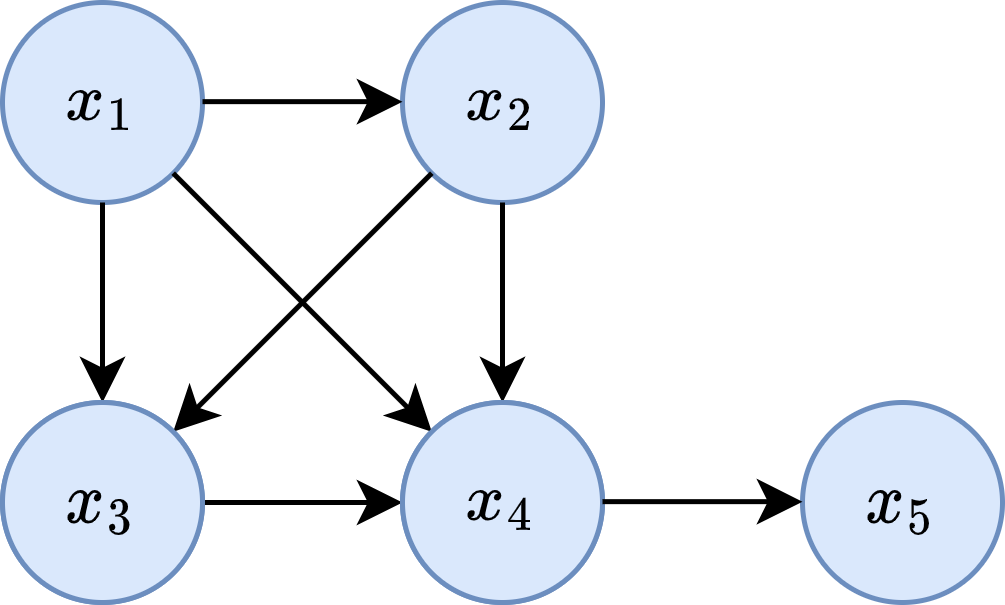
\includegraphics[width=0.5\linewidth]{images/draw.io/non_linear_scm.png}
	\caption{Non-Linear SCM $\mathcal{M}_{\text{NL}}$}
	\label{fig:non_linear_scm}
\end{figure}


\section{Evaluation Criteria} \comment{can probably ditch this section, consider have basically got rid of it}

To how useful the learned user preferences $\hat{\beta_k}$ and SCM approximation parameters $\hat{W}$ are, we need to be able to evaluate $\cost(\mathbf{x,x}^*)$, where $\mathbf{x}^*$ represents the recourse generated. To do this, we propose simply minimise the squared distance between the recourse $\mathbf{x}^*$ and $\mathbf{x}'$, which represents the parametric counterfactual from ordered actions $A$ under the true SCM. The objective function that is optimised is shown below.

\begin{equation}
	A^* = \argmin_{A} (\mathbf{x}^* - \mathbf{x}')^2
\end{equation}

where

\begin{align}
	A & = \big\{(\mathbf{S}, \text{do} \{\mathbf{x}'_i:=\mathbf{x}'_i + \boldsymbol{\delta}_i\}_{i=1, \ldots, D})\big\} \\ \nonumber
	{\mathbf{x}'}^{\text{PCF}} & = \mathbb{I}_{i \in I} \boldsymbol{\delta}_i + \bigg( \mathbf{x}'_i + f_i(\textbf{pa}^{\text{PCF}}_i) - f_i(\textbf{pa}_i) \bigg)
\end{align}

This can be optimised using gradient descent. Once we have obtained ordered actions $A^*$ that lead to our recourse $\mathbf{x}^*$ under the true SCM, we can calculate $\cost(\mathbf{x,x}')$ as $\cost(A^*, \beta_k, \mathcal{F})$ as defined in equation $\ref{eq:cost_function_experiments}$, where $\beta_k$ represents the true user preferences and $\mathcal{F}$ are the true structural equations.

\section{Results}

In this section, we present the results of the learned cost function on the two SCMs described in the previous section. In all the experiments conducted in this section, we simulate 2,000 individuals from the SCMs, which are then classified either positively or negatively.

\subsection{Linear SCM}

In this section, we detail the performance of our methodology on the linear SCM outlined in section \ref{section:linear_scm}. We compare the cost of the recourse we generated to the cost of the recourse generated using the ground truth user preferences $\beta_k$ and the ground truth SCM. Assuming that there is no noise in either the users' evaluation of their own preferences and their local evaluation of the SCM, we have calculated the percentage increase in cost of the recourse generated compared to the ground truth recourse.

\begin{table}[!htb]
	\centering
	\begin{tabular}{l|l|l}
		\hline
		\textbf{Model} & \textbf{Cost} & \textbf{Increase in cost (\%)} \\
		\hline
		Ground truth   & 0.214 & 0\%                        \\
		Identity $W$   & 0.363 & 69.5\%                     \\
		5 comparisons  & 0.332 &  55.1\%                     \\
		10 comparisons & 0.290 &  35.4\%                     \\
		20 comparisons & 0.250 &  16.7\%                     \\ 
		50 comparisons & 0.224 &  4.6\%                      \\ \hline
	\end{tabular}
	\caption{Ground truth cost of recourse }
\end{table}


\subsection{Non-Linear SCM}



================================================

[TO CLEAN UP]

\begin{figure}[!htb]
	\centering
	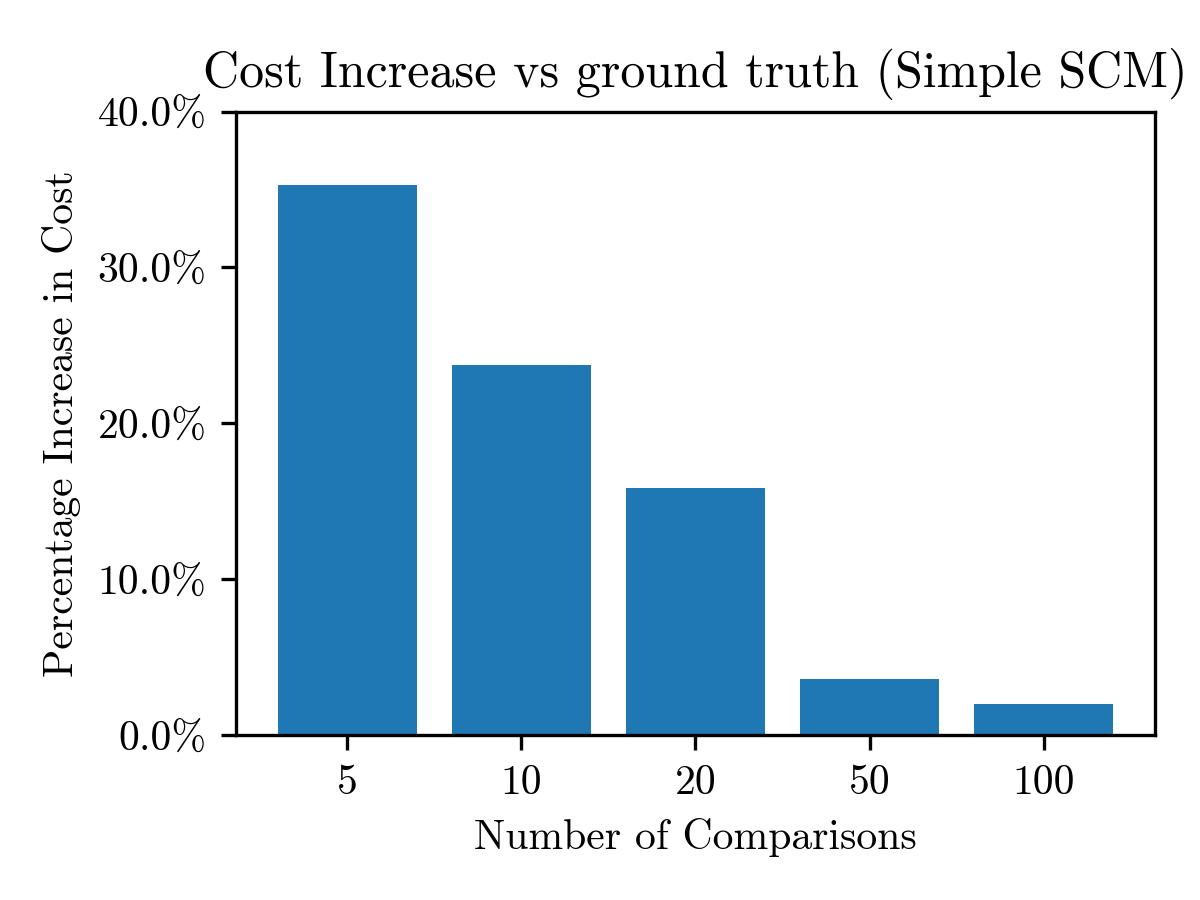
\includegraphics[scale=1]{images/simpleSCM_comparison_results.png}
	\caption{Comparison of the average cost of recourse for learned costs functions compared to the ground truth cost function for the Simple SCM.}
	\label{fig:simple_scm}
\end{figure}


\subsection{Noiseless responses with perfect knowledge of the causal graph}

Ground truth $\beta$: [0.5, 0.333, 0.1667] \\
Learned $\beta$ : [0.4965, 0.3355, 0.1681]

\subsection{Noiseless responses with imperfect knowledge of the causal graph}

Ground truth $\beta$: [0.5, 0.333, 0.1667] \\
Learned $\beta$ : [0.4975, 0.3354, 0.1671]

Ground truth $W$: $\begin{bmatrix}
	0 & 0.5 & 0.2 \\
	0 & 0 & 0.3 \\
	0 & 0 & 0
\end{bmatrix}$

Learned $W$: $\begin{bmatrix}
	0 & 0.4864 & 0.2136 \\
	0.0033 & 0 & 0.3221 \\
	0.0008 & 0.0086 & 0
\end{bmatrix}$



\subsection{Noisy responses}

So far, only noisy responses have been added (not noise knowledge of the causal graph)

\textbf{With noise distribution $N(0, 0.1)$:}

Ground truth $\beta$: [0.5, 0.333, 0.1667] \\
Learned $\beta$ : [0.4917, 0.3418, 0.1665]

Ground truth $W$: $\begin{bmatrix}
	0 & 0.5 & 0.2 \\
	0 & 0 & 0.3 \\
	0 & 0 & 0
\end{bmatrix}$

Learned $W$: $\begin{bmatrix}
	0 & 0.5424 & 0.1683 \\
	-0.0070 & 0 & 0.3950 \\
	0.0166 & -0.0007 & 0
\end{bmatrix}$


\textbf{With noise distribution $N(0, 0.5)$:}

Ground truth $\beta$: [0.5, 0.333, 0.1667] \\
Learned $\beta$ : [0.4224, 0.3686, 0.2090]

Ground truth $W$: $\begin{bmatrix}
	0 & 0.5 & 0.2 \\
	0 & 0 & 0.3 \\
	0 & 0 & 0
\end{bmatrix}$

Learned $W$: $\begin{bmatrix}
	0 & 0.5772 & 0.3522 \\
	-0.0062 & 0 & 0.1657 \\
	0.0974 & 0.0459 & 0
\end{bmatrix}$

\textbf{With noise distribution $N(0, 2)$:}

Ground truth $\beta$: [0.5, 0.333, 0.1667] \\
Learned $\beta$ : [0.4958, 0.2685, 0.2357]

Ground truth $W$: $\begin{bmatrix}
	0 & 0.5 & 0.2 \\
	0 & 0 & 0.3 \\
	0 & 0 & 0
\end{bmatrix}$

Learned $W$: $\begin{bmatrix}
	0 & 0.5353 & 0.08712 \\
	-0.1487 & 0 & 0.7206 \\
	-0.2152 & 0.2409 & 0
\end{bmatrix}$